%! TEX program = xelatex
% Paquetes:
\documentclass[letterpaper, 12pt]{article}
\usepackage[spanish]{babel} %%Paquete español para mac
\usepackage{graphicx} %% Para incluir figuras
\usepackage{xcolor}
\usepackage{ifpdf}
\usepackage{circledsteps}
\DeclareGraphicsExtensions{.pdf}
\usepackage[margin=1in]{geometry}
\setcounter{totalnumber}{5}
\renewcommand{\textfraction}{0.1}
\usepackage[cmex10]{amsmath}
\usepackage{amssymb}
\usepackage{float}
\usepackage{cite}
\bibliographystyle{unsrt}
%\decimalpoint
\usepackage{url}
\usepackage{hyperref}
\hypersetup{colorlinks=false,bookmarksopen=true,linkbordercolor={1 1 1}}
\usepackage{mathtools}
\usepackage{chngcntr}
\usepackage{enumitem}
\providecommand{\e}[1]{\ensuremath{\times 10^{#1}}}
\usepackage[parfill]{parskip} % Líneas en lugar de indentación
\usepackage{fancyhdr}
\usepackage{booktabs}
\usepackage{cleveref}
\usepackage{verbatimbox}
\crefformat{footnote}{#2\footnotemark[#1]#3}

\usepackage[squaren]{SIunits} %esto me da nombres de unidades y prefijos
\usepackage{sistyle}% Esto es adecuado para escribir unidades.

\newcommand{\alumno}{Agustín Campeny}
\lhead{\nouppercase{\leftmark}}
\rhead{Tarea 5 - \alumno}
\pagestyle{fancy}
%\usepackage{scrextend}
\numberwithin{equation}{section}

\setlength{\tabcolsep}{6pt} % General space between cols (6pt standard)
\renewcommand{\arraystretch}{0.8} % General space between rows (1 standard)
\begin{document}
\thispagestyle{empty}
%%%%%%%%%%%%%%%%%%%%%%%%%%
%%%%%%%%% ENCABEZADO %%%%%%%%%
%%%%%%%%%%%%%%%%%%%%%%%%%%
\vspace*{-1cm}

\includegraphics[width=2cm]{logo.pdf}
\vspace*{-2.2cm}

\hspace*{2cm}
 \begin{tabular}{l}
  {\ \textsc{\raggedright \footnotesize Pontificia Universidad Católica de Chile}}\\
  {\ \textsc{\raggedright \footnotesize Escuela de Ingeniería}}\\
  {\ \textsc{\raggedright \footnotesize Departamento de Ingeniería Eléctrica}}\\
  {\ \textsc{\raggedright \footnotesize IEE2753 - Diseño de Circuitos Integrados Digitales}}\\
  {\  }\\
 \end{tabular}
 \hfill
\vspace*{-0.2cm}
\begin{center}
  {\Large\bf Tarea 5}\\
\vspace*{2mm}
{\today}\\
\vspace*{2mm}
{\footnotesize \alumno}\\
\vspace*{6mm}
\end{center}
\hrule\vspace*{2pt}\hrule
%%%%%%%%%%%%%%%%%%%%%%%%%%
%%%%%%%%% ENCABEZADO %%%%%
%%%%%%%%%%%%%%%%%%%%%%%%%%

\section{Problemas: Retardo}

\subsection{Compuerta NAND4}

A continuación se presenta un bosquejo de la compuerta solicitada, junto con loas anchos para cada transistor, los que fueron escogidos para que el circuito tenga la misma resistencia en pullup y pulldown que el inversor descrito en el peor caso.

\begin{figure}[H]
  \centering
  % XCircuit output "1.1.tex" for LaTeX input from 1.1.eps
\def\putbox#1#2#3#4{\makebox[0in][l]{\makebox[#1][l]{}\raisebox{\baselineskip}[0in][0in]{\raisebox{#2}[0in][0in]{\scalebox{#3}{#4}}}}}
\def\rightbox#1{\makebox[0in][r]{#1}}
\def\centbox#1{\makebox[0in]{#1}}
\def\topbox#1{\raisebox{-0.60\baselineskip}[0in][0in]{#1}}
\def\midbox#1{\raisebox{-0.20\baselineskip}[0in][0in]{#1}}
   \scalebox{1}{
   \normalsize
   \parbox{3.03125in}{
   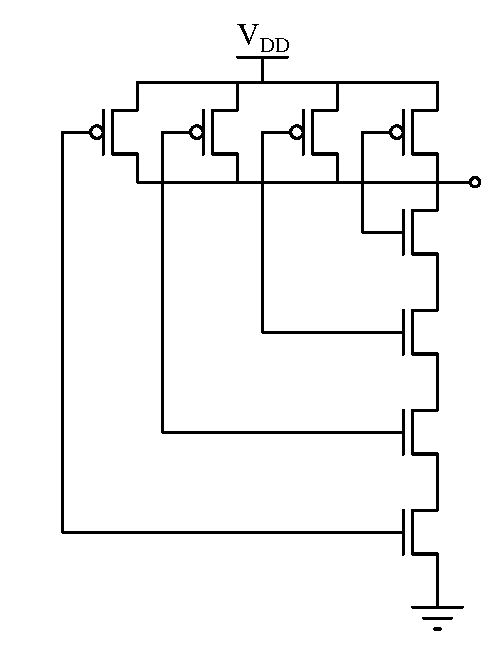
\includegraphics[scale=1]{1.1.eps}\\
   % translate x=656 y=636 scale 0.38
   \putbox{0.81in}{3.29in}{1.20}{2}%
   \putbox{1.47in}{3.29in}{1.20}{2}%
   \putbox{2.14in}{3.29in}{1.20}{2}%
   \putbox{2.81in}{3.29in}{1.20}{2}%
   \putbox{2.81in}{2.62in}{1.20}{4}%
   \putbox{2.81in}{1.95in}{1.20}{4}%
   \putbox{2.81in}{1.29in}{1.20}{4}%
   \putbox{2.81in}{0.62in}{1.20}{4}%
   \putbox{0.06in}{0.70in}{1.20}{A}%
   \putbox{0.72in}{1.37in}{1.20}{B}%
   \putbox{1.39in}{2.04in}{1.20}{C}%
   \putbox{2.06in}{2.70in}{1.20}{D}%
   } % close 'parbox'
   } % close 'scalebox'
   \vspace{-\baselineskip} % this is not necessary, but looks better

  \caption{Compuerta NAND4}
\end{figure}

\subsection{Compuerta NOR-N}

A continuación se presenta un bosquejo del circuito NOR de \(N\) entradas, con resistencia interna en subida y bajada igual a la de un inversor con \(W_p = 2\) y \(W_n = 1\).

\begin{figure}[H]
  \centering
  % XCircuit output "1.2.tex" for LaTeX input from 1.2.eps
\def\putbox#1#2#3#4{\makebox[0in][l]{\makebox[#1][l]{}\raisebox{\baselineskip}[0in][0in]{\raisebox{#2}[0in][0in]{\scalebox{#3}{#4}}}}}
\def\rightbox#1{\makebox[0in][r]{#1}}
\def\centbox#1{\makebox[0in]{#1}}
\def\topbox#1{\raisebox{-0.60\baselineskip}[0in][0in]{#1}}
\def\midbox#1{\raisebox{-0.20\baselineskip}[0in][0in]{#1}}
   \scalebox{1}{
   \normalsize
   \parbox{1.75521in}{
   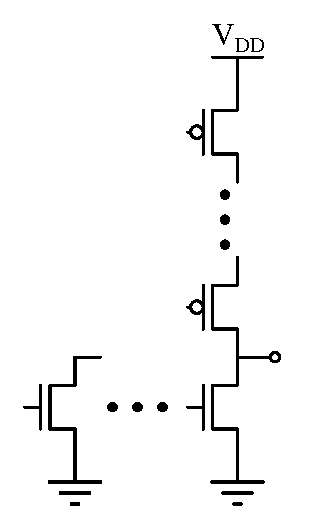
\includegraphics[scale=1]{1.2.eps}\\
   % translate x=496 y=540 scale 0.38
   \putbox{1.47in}{0.62in}{1.20}{1}%
   \putbox{0.39in}{0.62in}{1.20}{1}%
   \putbox{1.56in}{1.29in}{1.20}{2N}%
   \putbox{1.56in}{2.45in}{1.20}{2N}%
   } % close 'parbox'
   } % close 'scalebox'
   \vspace{-\baselineskip} % this is not necessary, but looks better

  \caption{Compuerta NOR-N}
\end{figure}

La capacitancia de entrada del inversor unitario es de \(3C\), y su retardo parasitario \(\tau_{inv} = 3RC\). Es posible notar que cada entrada del NOR-N ve una capacitancia de \((2N + 1)C\) unidades, por lo tanto su esfuerzo lógico es de \(g = (2N+1)/3\).

Por como se definieron los anchos, la capacitancia del nodo de salida del NOR-N es de \(3NC\), y la resistencia es \(R\), por lo tanto \(t_{pd} = 3NRC\), y su restraso relativo al inversor unitario es \(d = t_{pd} / \tau_{inv} =  N\).

\subsection{CMOS Complementaria}

\subsubsection{}

Como la resistencia del PMOS es igual a la mitad de la resistencia del NMOS, para lograr igual resistencia de pullup y pulldown, el valor de \(W_p = 1\) y \(W_n = 2\).

\subsubsection{}

Se presenta el circuito que corresponde a la función \(F = \overline{((A+B)\cdot C + D)\cdot E}\).

\begin{figure}[H]
  \centering
  % XCircuit output "1.3.tex" for LaTeX input from 1.3.eps
\def\putbox#1#2#3#4{\makebox[0in][l]{\makebox[#1][l]{}\raisebox{\baselineskip}[0in][0in]{\raisebox{#2}[0in][0in]{\scalebox{#3}{#4}}}}}
\def\rightbox#1{\makebox[0in][r]{#1}}
\def\centbox#1{\makebox[0in]{#1}}
\def\topbox#1{\raisebox{-0.60\baselineskip}[0in][0in]{#1}}
\def\midbox#1{\raisebox{-0.20\baselineskip}[0in][0in]{#1}}
   \scalebox{1}{
   \normalsize
   \parbox{2.78125in}{
   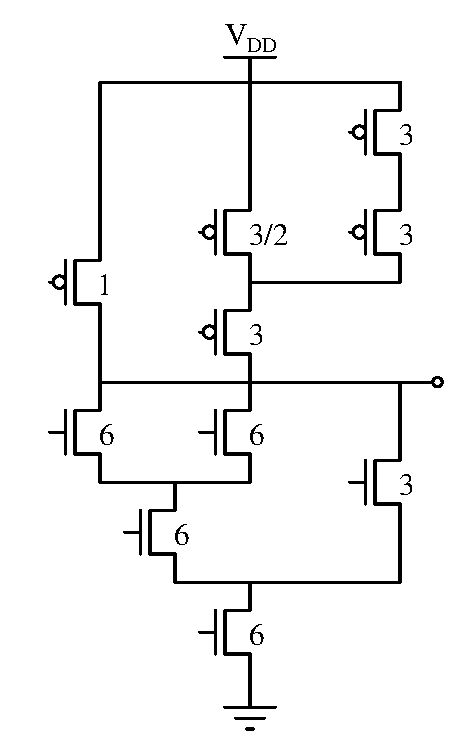
\includegraphics[scale=1]{1.3.eps}\\
   % translate x=544 y=732 scale 0.38
   \putbox{2.06in}{3.95in}{1.20}{A}%
   \putbox{2.06in}{3.29in}{1.20}{B}%
   \putbox{1.06in}{3.29in}{1.20}{C}%
   \putbox{1.06in}{2.62in}{1.20}{D}%
   \putbox{0.06in}{2.95in}{1.20}{E}%
   \putbox{0.06in}{1.95in}{1.20}{A}%
   \putbox{1.06in}{1.95in}{1.20}{B}%
   \putbox{2.06in}{1.62in}{1.20}{D}%
   \putbox{0.56in}{1.29in}{1.20}{C}%
   \putbox{1.06in}{0.62in}{1.20}{E}%
   } % close 'parbox'
   } % close 'scalebox'
   \vspace{-\baselineskip} % this is not necessary, but looks better

  \caption{Compuerta F}
\end{figure}

Las medidas fueron escogidas para que los peores casos de pullup y pulldown sean tengan la misma resistencia interna que la del inversor unitario definido en el item anterior.

\subsubsection{}

La capacitancia de entrada del inversor unitario corresponde a \(3C\), mientras que la capacitancia de entrada para el circuito \(F\) de la entrada \(E\) es \(7C\). De este modo, el \emph{logical effort} de la entrada \(E\) es \(g_E = 7/3\).

\subsection{AND-OR-INVERTER}

Primero para estimar la capacitancia de cada nodo, se utiliza la convención de que la difusión con contacto tiene una capacitancia \(C_g\cdot W\), mientras que la la difusión combinada, que es el caso de transistores en serie, tiene la mitad, o sea \(C_g\cdot W/2\).

\begin{figure}[H]
  \centering
  % XCircuit output "1.4a.tex" for LaTeX input from 1.4a.eps
\def\putbox#1#2#3#4{\makebox[0in][l]{\makebox[#1][l]{}\raisebox{\baselineskip}[0in][0in]{\raisebox{#2}[0in][0in]{\scalebox{#3}{#4}}}}}
\def\rightbox#1{\makebox[0in][r]{#1}}
\def\centbox#1{\makebox[0in]{#1}}
\def\topbox#1{\raisebox{-0.60\baselineskip}[0in][0in]{#1}}
\def\midbox#1{\raisebox{-0.20\baselineskip}[0in][0in]{#1}}
   \scalebox{1}{
   \normalsize
   \parbox{2.15104in}{
   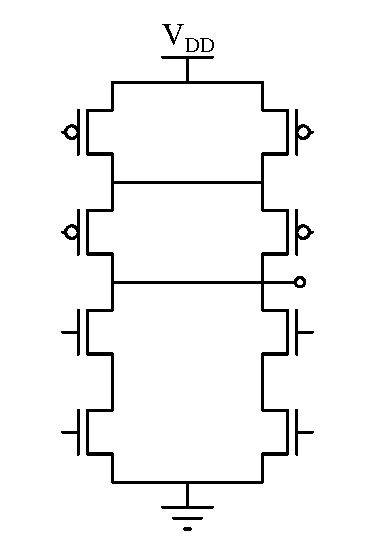
\includegraphics[scale=1]{1.4a.eps}\\
   % translate x=416 y=476 scale 0.38
   \putbox{0.06in}{1.95in}{1.20}{A}%
   \putbox{2.06in}{1.95in}{1.20}{B}%
   \putbox{0.06in}{2.62in}{1.20}{C}%
   \putbox{2.06in}{2.62in}{1.20}{D}%
   \putbox{0.06in}{1.29in}{1.20}{A}%
   \putbox{0.06in}{0.62in}{1.20}{B}%
   \putbox{2.06in}{1.29in}{1.20}{C}%
   \putbox{2.06in}{0.62in}{1.20}{D}%
   } % close 'parbox'
   } % close 'scalebox'
   \vspace{-\baselineskip} % this is not necessary, but looks better

  \caption{Compuerta AOI4}
\end{figure}

Se puede notar que si bien los PMOS de ambas ramas se encuentran en serie, estas tienen un contacto, por lo tanto el nodo considera las capacitancias de ambas difusiones. Los NMOS serie poseen difusiones combinadas, por lo tanto presentan la mitad de la capacitancia, y el nodo de salida corresponde a la suma de las difusiones con contacto PMOS y NMOS.

\begin{figure}[H]
  \centering
  % XCircuit output "1.4b.tex" for LaTeX input from 1.4b.eps
\def\putbox#1#2#3#4{\makebox[0in][l]{\makebox[#1][l]{}\raisebox{\baselineskip}[0in][0in]{\raisebox{#2}[0in][0in]{\scalebox{#3}{#4}}}}}
\def\rightbox#1{\makebox[0in][r]{#1}}
\def\centbox#1{\makebox[0in]{#1}}
\def\topbox#1{\raisebox{-0.60\baselineskip}[0in][0in]{#1}}
\def\midbox#1{\raisebox{-0.20\baselineskip}[0in][0in]{#1}}
   \scalebox{1}{
   \normalsize
   \parbox{3.58333in}{
   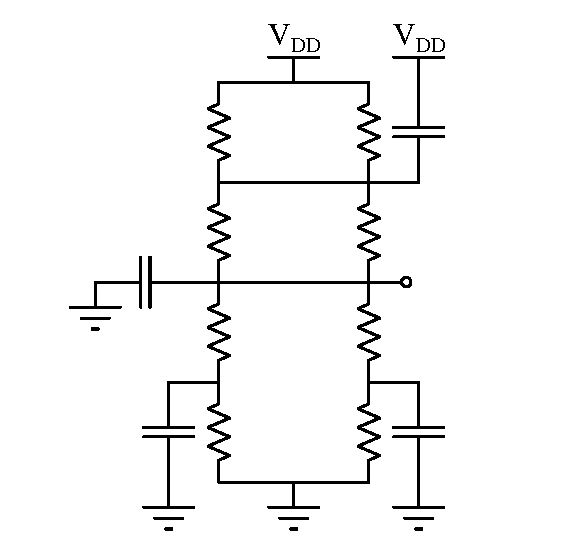
\includegraphics[scale=1]{1.4b.eps}\\
   % translate x=632 y=540 scale 0.38
   \putbox{2.93in}{2.62in}{1.20}{\(2C_gW_p\)}%
   \putbox{2.93in}{0.62in}{1.20}{\(\frac{C_gW_p}{2}\)}%
   \putbox{0.76in}{0.62in}{1.20}{\rightbox{\(\frac{C_gW_p}{2}\)}}%
   \putbox{1.18in}{1.95in}{1.20}{\rightbox{\(C_g(W_p+W_n)\)}}%
   \putbox{1.43in}{2.62in}{1.20}{$R_p$}%
   \putbox{1.43in}{1.95in}{1.20}{$R_p$}%
   \putbox{2.01in}{2.62in}{1.20}{$R_p$}%
   \putbox{2.01in}{1.95in}{1.20}{$R_p$}%
   \putbox{1.43in}{1.29in}{1.20}{$R_n$}%
   \putbox{2.01in}{1.29in}{1.20}{$R_n$}%
   \putbox{1.43in}{0.62in}{1.20}{$R_n$}%
   \putbox{2.01in}{0.62in}{1.20}{$R_n$}%
   } % close 'parbox'
   } % close 'scalebox'
   \vspace{-\baselineskip} % this is not necessary, but looks better

  \caption{Circuito equivalente}
\end{figure}

En el circuito equivalente \(R_p = 2R/W_p\) y \(R_n = R/W_n\). Se determinan los retrasos de propagación ascendentes y descendentes para los peores casos.

Para el caso ascendente, el peor caso corresponde a \(A,C=1\) y \(B,D=1\rightarrow 0\), ya que como el NMOS C sigue conduciendo, su capacitancia de difusión contribuye a la capacitancia en la salida. Se determina el retraso:

\begin{align}
  t_{pdr} &= \frac{2R}{W_p}\cdot 2C_gW_p + \frac{4R}{W_p}\left( C_g(W_p+W_n) + C_gW_n/2 \right) \\
          &= 4RC_g\left( \frac{3}{2}\frac{W_n}{W_p}+2 \right)
\end{align}

El peor caso de retraso descendente se da cuando \(A,B=0\) y \(C,D=0\rightarrow 1\), ya que la capacitancia del nodo entre difusiones PMOS contribuye a la capacitancia de salida. Se determina el retraso:

\begin{align}
  t_{pdf} &= \frac{R}{W_n}\cdot \frac{C_gW_n}{2} + \frac{2R}{W_n}\left( C_g (W_p+W_n) + 2C_gW_p\right) \\
          &= 2RC_g\left( 3\frac{W_p}{W_n} + \frac{5}{2}\right)
\end{align}

\subsection{Compuerta CMOS}

\subsubsection{}

Se presenta un bosquejo del circuito descrito, con una resistencia interna determinada para los peores casos.

\begin{figure}[H]
  \centering
  % XCircuit output "1.5.1.tex" for LaTeX input from 1.5.1.eps
\def\putbox#1#2#3#4{\makebox[0in][l]{\makebox[#1][l]{}\raisebox{\baselineskip}[0in][0in]{\raisebox{#2}[0in][0in]{\scalebox{#3}{#4}}}}}
\def\rightbox#1{\makebox[0in][r]{#1}}
\def\centbox#1{\makebox[0in]{#1}}
\def\topbox#1{\raisebox{-0.60\baselineskip}[0in][0in]{#1}}
\def\midbox#1{\raisebox{-0.20\baselineskip}[0in][0in]{#1}}
   \scalebox{1}{
   \normalsize
   \parbox{2.27083in}{
   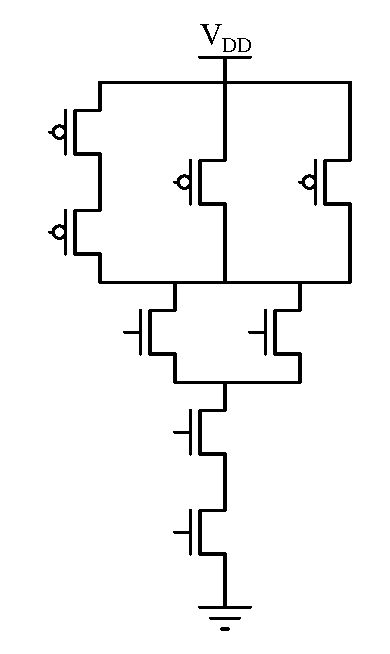
\includegraphics[scale=1]{1.5.1.eps}\\
   % translate x=448 y=700 scale 0.38
   \putbox{0.06in}{3.29in}{1.20}{A}%
   \putbox{0.06in}{2.62in}{1.20}{B}%
   \putbox{0.89in}{2.95in}{1.20}{C}%
   \putbox{1.72in}{2.95in}{1.20}{D}%
   \putbox{0.56in}{1.95in}{1.20}{A}%
   \putbox{1.39in}{1.95in}{1.20}{B}%
   \putbox{0.89in}{1.29in}{1.20}{C}%
   \putbox{0.89in}{0.62in}{1.20}{D}%
   \putbox{0.56in}{3.29in}{1.20}{8}%
   \putbox{0.56in}{2.62in}{1.20}{8}%
   \putbox{1.39in}{2.95in}{1.20}{4}%
   \putbox{2.22in}{2.95in}{1.20}{4}%
   \putbox{1.06in}{1.95in}{1.20}{6}%
   \putbox{1.89in}{1.95in}{1.20}{6}%
   \putbox{1.39in}{1.29in}{1.20}{6}%
   \putbox{1.39in}{0.62in}{1.20}{6}%
   } % close 'parbox'
   } % close 'scalebox'
   \vspace{-\baselineskip} % this is not necessary, but looks better

  \caption{Circuito descrito por la función \(F\)}
\end{figure}

\subsubsection{}

Una manera sencilla de mejorar este camino crítico, es posicionando los transistores que son controlados por \(A\) lo mas cercano a la salida. De forma práctica, colocar el PMOS manejado por \(A\) por debajo del PMOS de \(B\) aportaría a disminuir el retraso del camino.

\subsection{Buffers}

Los datos entregados en el enunciado se utilizan para obtener las capacitancias de compuerta y difusión de cada etapa. Primero se determina la capacitancia de entrada y difusión de la primera etapa de inversor:

\begin{equation}
  C_{in1} = C_{out1} = C_D\cdot (12\lambda + 6\lambda) = \SI{0.486}{fF}
\end{equation}

Luego se obtiene el valor de \emph{Path Effort} \(F = GBH\). Como no existen ramificaciones el valor de \(B = 1\), y como todas las compuertas corresponden a inversores mínimos escalados, el valor de \(G = 1\). Finalmente \(F = H\), y por lo tanto:

\begin{equation}
  F = H = \frac{C_{Load}}{C_{in1}} = \frac{\SI{518}{fF}}{\SI{0.486}{fF}} \approx 1066
\end{equation}

Ya con estos valores es posible conseguir las medidas de los inversores intermedios que minimizan el retraso total del camino. Para esto se determina el valor del \emph{Best Stage Effort} \(\hat{f}\):

\begin{equation}
  \hat{f} = \sqrt[n]{F} = \sqrt[4]{1066} \approx 5.71
\end{equation}

Finalmente, se multiplican las medidas de cada etapa por \(\hat{f}\) para obtener la siguiente, y así las medidas finales son las siguientes:

\begin{equation}
  1:12\lambda/6\lambda \quad 2:68.5\lambda/34.3\lambda \quad 3: 391.1\lambda/195.9\lambda \quad 4:2233.2\lambda/1118.6\lambda
\end{equation}

Asumiendo la etapa 1 como el inversor unitario, se calcula el retardo total normalizado:

\begin{equation}
  D = n\sqrt[n]{F} + p = 26.84
\end{equation}

La resistencia interna del inversor unitario es igual para el PMOS y el NMOS, ya que el PMOS tiene el doble de ancho, y es igual a:

\begin{equation}
  R = \frac{2}{6}\cdot \SI{13}{k\Omega/\square} = \SI{4.33}{\Omega}
\end{equation}

La capacitancia es:

\begin{equation}
  C = (12 + 6)\delta \cdot C_D = \SI{0.486}{fF}
\end{equation}

El retardo del inversor unitario es \(\tau = RC = \SI{2.11}{ps}\), y así finalmente el retardo total del circuito es \(t_{pd} = D\tau = \SI{56.63}{ps}\).

\subsection{Branching effort}

\subsubsection{}

Para el circuito del enunciado, se tienen 8 bifurcaciones idénticas, por lo tanto \(B = 8\). Utilizando los esfuerzos lógicos estándar para las compuertas NAND y NOR del camino, se determina \(G = 4/3\cdot 5/3 = 20/9\). Finalmente la capacitancia de carga es de \SI{200}{fF}, y la capacitancia de la primera etapa es de \SI{10}{fF}, asi que \(H = 200/10 = 20\). Con esta información, el \emph{path effort} para cualquier camino es:

\begin{equation}
  F = GBH \approx 356
\end{equation}

\subsubsection{}

El valor de \(\hat{f} = \sqrt[4]{F} \approx 4.34 \), y con este ya es posible determinar la capacitancia de entrada de cada compuerta. Comenzando desde el final del path:

\begin{gather}
  C_{in4} = \frac{\SI{200}{fF}\cdot 1}{4.34} \approx \SI{46.10}{fF} \\
  C_{in3} = \frac{\SI{46.10}{fF}\cdot 5/3}{4.34} \approx \SI{17.70}{fF} \\
  C_{in2} = \frac{\SI{17.70}{fF}\cdot 4/3 \cdot 8}{4.34} \approx \SI{43.50}{fF} \\
  C_{in1} = \frac{\SI{43.50}{fF}\cdot 1}{4.34} \approx \SI{10}{fF}
\end{gather}

Como se logró llegar a la capacitancia de la etapa inicial, los valores fueron correctamente asignados. El inversor final tiene una capacitancia de entrada de \(C_{in4} = \SI{46.10}{fF}\), y la compuerta NOR tiene \(C_{in3} = \SI{46.10}{fF}\).







\end{document}
